\section{MY ONLY SECTION}

	\ifCLASSOPTIONjournal
		\IEEEPARstart{J}{urnals} use this convention for the first letter of a journal paper.
	\else
		Conference papers use normal size for the first letter of the conference paper.
	\fi	

The \ac{iot} is becoming very popular. One of the elements of \ac{iot} are embedded systems. There is a lot of \aclp{iot} devices currently on the market the acronym for them is \acsp{iot}.

On the \acf{fri} you will learn about \acs{ram} which is short for \acl{ram}.

The monkeys are very smart animals \cite{article_first}. They are shown in \figurename ~\ref{fig:monkey}. 

% Remember, if you use \IEEEpubid you must call \IEEEpubidadjcol in the second and first
% column for its text to clear the IEEEpubid mark.
\IEEEpubidadjcol

\begin{figure}[ht]
	\centering
	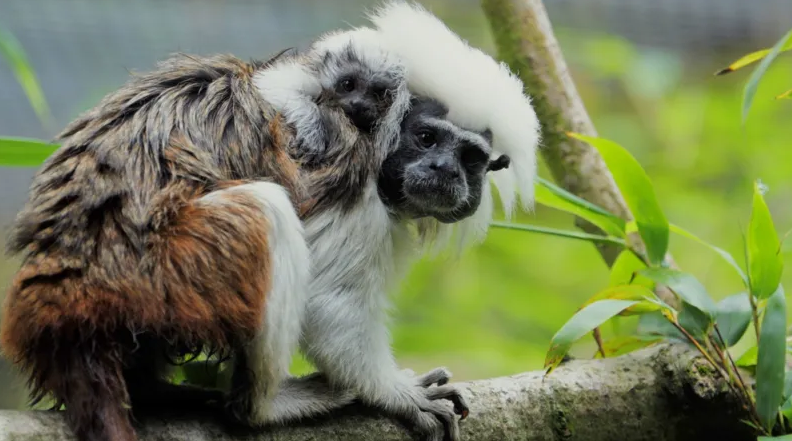
\includegraphics[width=1.0\linewidth]{pictures/monkey}
	\caption{Nice picture of monkey \cite{figure_first}}
	\label{fig:monkey}
\end{figure}


We can use vibrational energy harvesting during monkey studies \cite{article_second}. Its basic principle is shown in \figurename  ~\ref{fig:vibrationalenergyharvesting}.

\begin{figure}[ht]
	\centering
	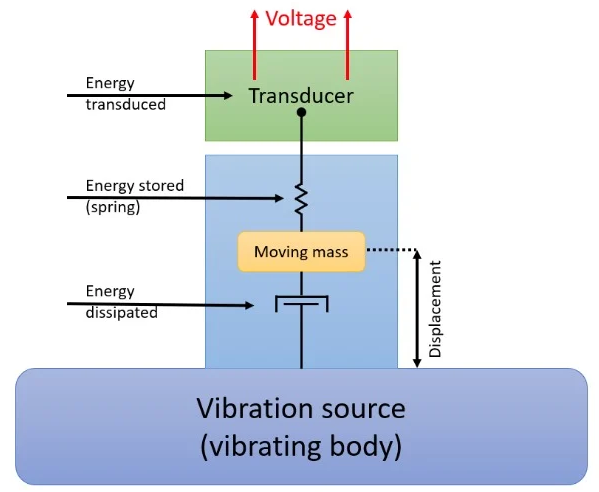
\includegraphics[width=1.0\linewidth]{pictures/vibrational_energy_harvesting}
	\caption{Vibrational energy harvesting principle \cite{figure_second}}
	\label{fig:vibrationalenergyharvesting}
\end{figure}

This is how you should cite text that has multiple sources \cite{article_first, article_second}.

In table \ref{tab:first_table} we have some measured data.

\begin{table}[ht]
	\centering
	\caption{My first table}
	\label{tab:first_table}
	\begin{tabular}{|c|c|c|c|}
		\hline
		& $a$ & $b$ & $c$ \\
		\hline
		$a$ & 1 & 0 & 1 \\
		\hline
		$b$ & 0 & 1 & 1 \\
		\hline
		$c$ & 1 & 1 & 0 \\
		\hline
	\end{tabular}
\end{table}

And in the \eqref{eq:original_equation} is shown a very simple formula. Based on which the variable $a$ is a sum of two variables $b$ and $c$.

\begin{equation}
	\label{eq:original_equation}
	a = b + c
\end{equation}

We can also calculate the value of variable $c$ by altering the equation as in \eqref{eq:altered_equation}. 

\begin{equation}
	\label{eq:altered_equation}
	c = a - b
\end{equation}



% Remember, if you use \IEEEpubid you must call \IEEEpubidadjcol in the second and first
% column for its text to clear the IEEEpubid mark.
\IEEEpubidadjcol

This way we can create a plain unnumbered list.

\begin{list}{}{}
	\item Hope
	\item Elizabeth
	\item Josette 
\end{list}

This way we can create an unnumbered list.

\begin{itemize}
	\item Hope
	\item Elizabeth
	\item Josette
\end{itemize}

This way we can create an numbered list.

\begin{enumerate} 
	\item Hope
	\item Elizabeth
	\item Josette
\end{enumerate}

This way we can create lists with descriptions.

\begin{description}
	\item[red] nice colour
	\item[blue] not very nice colour
\end{description}

